\title{คาบเรียนที่ 13: การหาปริพันธ์โดยการแยกเศษส่วนย่อย และการแทนค่าในรูปตัวแปรใหม่}
\frame{\titlepage}

\begin{frame}
\frametitle{สารบัญ}
\tableofcontents
\end{frame}

\begin{frame}
\frametitle{ที่มา}
เราสามารถใช้การแทนค่า $u$ เพื่อหาปริพันธ์ได้ ถ้าฟังก์ชันอยู่ในรูปแบบที่คุ้นเคย เช่น
\[\sin u, \quad \cos u, \quad \tan u, \quad e^u, \quad \ln u, \quad \sinh u, \ldots\]
ในบทนี้ เราจะเรียนรูปแบบการแทนค่า $u$ เช่นกัน แต่ $u$ ของเราจะไม่มีรูปแบบตายตัว ต้องดูรูปแบบจากโจทย์ โดยจะศึกษาทั้งหมด 2 รูปแบบด้วยกัน ได้แก่

\tableofcontents

ถ้าโจทย์ปริพันธ์ไม่ตรงกับรูปแบบที่เราเคยศึกษา เช่น $\int \sin (x^2 )\, dx$ ให้นับว่าเรายังไม่สามารถแก้ได้ด้วยความรู้แคลคูลัส 1
\end{frame}


%%%%%%%%%%%%%%
\section[เศษส่วนพหุนาม]{ปริพันธ์ของฟังก์ชันเศษส่วนพหุนาม}
\frame{\sectionpage}
%%%%%%%%%%%%%%

\begin{frame}[t]
\frametitle{ที่มา}
ถ้าปริพันธ์อยู่ในรูปเศษส่วนพหุนาม
\begin{block}{}
\[ \int \frac{P(x)}{Q(x)} \, dx\] 
\end{block}
โดยที่ดีกรี (เลขชี้กำลังของพจน์ที่สูงที่สุด) ของ $P(x)$ มากกว่า $Q(x)$ แล้วให้ใช้การหารพหุนาม
\begin{slide}
\[P(x) = F(x)Q(x) + R(x)\]
โดยที่ $F(x)$ และ $R(x)$ เป็นพหุนาม จากนั้นจึงสามารถจัดรูปได้ดังนี้
 \[\int \frac{P(x)}{Q(x)} \, dx = \int \frac{F(x)Q(x) + R(x)}{Q(x)} \, dx = \int F(x) + \frac{R(x)}{Q(x)} \, dx\]
 จากนั้นจึงหาปริพันธ์แยกกัน
 \end{slide}
\end{frame}


\begin{frame}[t]
\begin{ex} 
จงหาปริพันธ์ $\int \frac{x^2}{x-1} \, dx$
\end{ex}
\begin{sol}
หาผลหารของพหุนาม $x^2$ ด้วย $\red{x-1}$ ได้ดังนี้
\[x^2 = (x^2-1) + 1 = (x+1)\red{(x-1)} + 1\]
ดังนี้
\begin{eq*}
\int \frac{x^2}{x-1} \, dx &=& \int \frac{(x+1)(x-1) + 1}{x-1} \, dx \\
&=& \int (x+1) + \frac{1}{x-1} \, dx \\
&=& \int (x+1) \, dx + \int \frac{1}{x-1} \, dx \\
&=& \tfrac{1}{2}x^2 + x + \ln|x-1| + C
\end{eq*}
\end{sol}
\end{frame}


\begin{frame}[t]
\begin{ex} 
จงหาปริพันธ์ $\int \frac{x^4+1}{x^2+1} \, dx$
\end{ex}
\begin{sol}
หาผลหารของพหุนาม $x^4+1$ ด้วย $\red{x^2+1}$ ได้ดังนี้
\[x^4+1 = (x^4-1) + 2 = (x^2-1)\red{(x^2+1)} + 2\]
ดังนี้
\begin{eq*}
\int \frac{x^4+1}{x^2+1} \, dx &=& \int \frac{(x^2-1)(x^2+1) + 2}{x^2+1} \, dx \\
&=& \int (x^2-1) + \frac{2}{x^2+1} \, dx \\
&=& \int (x^2-1) \, dx + 2\int \frac{1}{x^2+1} \, dx \\
&=& \tfrac{1}{3}x^3 - x + 2\arctan{x} + C
\end{eq*}
\end{sol}
\end{frame}

%%%%%%%%%%%%%%
\section[เศษส่วนย่อย]{การแยกเศษส่วนย่อย}
\frame{\sectionpage}
%%%%%%%%%%%%%%

\begin{frame}[t]
\frametitle{ที่มาของการแยกเศษส่วนย่อย}
ถ้าปริพันธ์อยู่ในรูปเศษส่วนพหุนาม $\int \frac{P(x)}{Q(x)} \, dx$ \red{แต่}ดีกรี ของ $P(x)$ น้อยกว่า $Q(x)$ และไม่มีอยู่ในรูปแบบของสูตรที่เคยศึกษามาแล้ว ต้องใช้ทฤษฎีบทต่อไปนี้
\begin{thm}{}{}
ถ้าแยกตัวประกอบ $Q(x)$ ได้เป็น $Q(x) = (x-a_1)(x-a_2)\ldots(x-a_n)$ เมื่อ $a_1,a_2,\ldots,a_n$ ไม่ซ้ำกัน แล้ว \pa
\[ \frac{P(x)}{Q(x)} = \frac{A_1}{x-a_1} + \frac{A_2}{x-a_2} + \cdots + \frac{A_n}{x-a_n}\] \pa
เมื่อ $A_1, A_2, \ldots, A_n$ เป็นค่าคงตัว 
\end{thm}
\end{frame}

\begin{frame}[t]
ในกรณีที่ $Q(x)$ เป็นพหุนามอันดับ 2 นั่นคือ เราสามารถแยกตัวประกอบได้เป็น $Q(x) = (x-a)(x-b)$ จะได้ว่า \pa 
\begin{slide}
\[ \frac{P(x)}{(x-a)(x-b)} = \frac{A}{x-a} + \frac{B}{x-b}\] \pa
ซึ่งเมื่อคูณทั้งสองฝั่งของสมการด้วย $(x-a)(x-b)$ จะได้ \pa
\[ P(x) = A(x-b) + B(x-a)\] \pa
ถ้าเราแทนค่า $\red{x=a}$ ในสมการจะได้ \pa
\[ P(\red{a}) = A(\red{a}-b) + B(\red{a}-a) = A(\red{a}-b)\] \pa
ฉะนั้น เราจะได้ $A = \frac{P(a)}{a-b}$ \pa ในทำนองเดียวกัน ถ้าแทนค่า $\blue{x=b}$ จะได้ \pa
\[P(\blue{b}) = A(\blue{b}-b) + B(\blue{b}-a) = B(\blue{b}-a)\] \pa
นั่นคือ $B = \frac{P(b)}{b-a}$  \pa
\end{slide}
\end{frame}


\begin{frame}[t]
\begin{ex} 
จงแปลง $\frac{1}{x(x-1)}$ ให้เป็นเศษส่วนย่อย \label{ex:partial_fraction1}
\end{ex}
\begin{sol}
กำหนดให้  $\frac{1}{x(x-1)} = \frac{A}{x} + \frac{B}{x-1}$ \pa
เมื่อคูณทั้งสองฝั่งของสมการด้วย $x(x-1)$ จะได้ \pa
\[1 = A(x-1) + Bx \] \pa
เมื่อแทนค่า $\red{x=0}$ และ $\blue{x=1}$ ดังต่อไปนี้ \pa
\[ 1 = A(\red{0}-1) + B (\red{0})= -A \qquad  \Longrightarrow \qquad A = -1\] 
\[1 = A(\blue{1}-1) + B(\blue{ 1}) = B \qquad \Longrightarrow \qquad B = 1\]  
ดังนั้น $ \frac{1}{x(x-1)} = \frac{-1}{x} + \frac{1}{x-1}$
\end{sol}
\end{frame}


\begin{frame}[t]
\begin{ex}
จงแปลง $\frac{3x}{(x-2)(x+4)}$ ให้เป็นเศษส่วนย่อย \label{ex:partial_fraction2}
\end{ex}
\begin{sol}
ถ้าเราต้องการเปลี่ยน $\frac{3x}{(x-2)(x+4)}$ เป็นเศษส่วนย่อย นั่นคือ $\frac{x}{(x-2)(x+4)} = \frac{A}{x-2} + \frac{B}{x+4}$ \pa
เมื่อคูณทั้งสองฝั่งของสมการด้วย $(x-2)(x+4)$ จะได้ \pa 
\[3x = A(x+4) + B(x-2) \] \pa
เมื่อแทนค่า $\red{x=2}$ และ $\blue{x=-4}$ (เพื่อทำให้พจน์ $B$ หายไป) จะได้\pa 
\[6 = A(\red{2}+4) + B(\red{2}-2) = 6A \qquad \Longrightarrow \qquad A = 1\] 
\[-12 = A(\blue{-4}+4) + B(\blue{-4}-2) = -6B \qquad \Longrightarrow \qquad B = 2\] 
ดังนั้น $ \frac{x}{(x-2)(x+4)} = \frac{1}{x-2} + \frac{2}{x+4}$
\end{sol}
\end{frame}


%%%%%%%%%%%%%%
\section{การหาปริพันธ์โดยการแยกเศษส่วนย่อย}
\frame{\sectionpage}
%%%%%%%%%%%%%%

\begin{frame}
\frametitle{การหาปริพันธ์เมื่อแยกเป็นเศษส่วนย่อยได้แล้ว}
เมื่อเราแยกเป็นเศษส่วนย่อยได้สำเร็จแล้ว เราก็จะสามารถหาปริพันธ์ได้ด้วยสูตร
\[ \int \frac{1}{x} \, dx = \begin{slide}\ln |x| + C\end{slide} \] \pa
ซึ่งเราสามารถใช้การแทนค่า $u$ เพื่อขยายเป็นสูตรทั่วไปได้ดังนี้ \pa
\begin{thm}{}{}
ให้ $r,s$ เป็นจำนวนจริง โดยที่ $r \neq 0$ จะได้ว่า
\begin{equation} \label{eq:integral_fraction}
 \int \frac{1}{rx + s} \, dx = \frac{1}{r} \ln |rx+s| + C
 \end{equation}
\end{thm}
\end{frame}

\begin{frame}
\begin{sol}
ให้เทคนิคการแทนค่า $u$ โดยให้ $u = rx + s$ จะได้ $du = r \, dx$ ดังนั้น\pa
\begin{eqnarray*}
\int \frac{1}{rx+s} \, dx \pa &=& \int \frac{1}{u} \left(\frac{du}{r}\right) \\
\pa &=& \frac{1}{r} \int \frac{1}{u} \, du \\
\pa &=& \frac{1}{r} \ln |u| + C \pa = \frac{1}{r} \ln |rx+s| + C
\end{eqnarray*}
\end{sol}
\end{frame}


\begin{frame}[t]
\begin{ex}
จงใช้สมการ \eqref{eq:integral_fraction} เพื่อหาปริพันธ์ต่อไปนี้
\begin{tasks}(3)
\task $\int \frac{1}{x-4} \, dx$
\task $\int \frac{1}{2x+3} \, dx $
\task $\int \frac{1}{-5x+4} \, dx $
\end{tasks}
\end{ex}
\begin{sol}
\begin{tasks}(1)
\task $\int \frac{1}{x-4} \, dx = \ln |x-4| + C$
\task $\int \frac{1}{2x+3} \, dx = \frac{1}{2} \ln | 2x+3 | + C$
\task $\int \frac{1}{-5x+4} \, dx = \frac{1}{-5} \ln | - 5x + 4| + C$
\end{tasks}
\end{sol}
\end{frame}



\begin{frame}[t]
\begin{ex}
จงหา $\int \frac{1}{x(x-1)} \, dx$
\end{ex}
\begin{sol}
จากตัวอย่างในหน้าที่ \ref{ex:partial_fraction1} เราสามารถแยกเป็นเศษส่วนย่อยดังนี้
\[\frac{1}{x(x-1)} = -\frac{1}{x} + \frac{1}{x-1}\] \pa
ฉะนั้น
\begin{eqnarray*}
\int \frac{1}{x(x-1)} \, dx \pa &=& \int \left(- \frac{1}{x} + \frac{1}{x-1} \right)\, dx \\
\pa &=& - \int \frac{1}{x} \, dx + \int \frac{1}{x-1} \, dx \\
\pa &=& - \ln |x| + \ln |x-1| + C
\end{eqnarray*}
\end{sol}
\end{frame}


\begin{frame}[t]
\begin{ex}
จงหา $\int \frac{3x}{(x-2)(x+4)} \, dx$
\end{ex}
\begin{sol}
จากตัวอย่างในหน้าที่ \ref{ex:partial_fraction2} เราสามารถแยกเป็นเศษส่วนย่อยดังนี้
\[\frac{3x}{(x-2)(x+4)} = \frac{1}{x-2} + \frac{2}{x+4}\] \pa
ฉะนั้น
\begin{eqnarray*}
\int \frac{x}{(x-2)(x+4)} \, dx \pa &=& \int \left( \frac{1}{x-2} + \frac{2}{x+4} \right)\, dx \\
\pa &=& - \int \frac{1}{x-2} \, dx + 2\int \frac{1}{x+4} \, dx \\
\pa &=& \ln |x-2| + 2\ln |x+4| + C
\end{eqnarray*}
\end{sol}
\end{frame}


\begin{frame}[t]
\begin{ex}
จงหา $\int \frac{2x+4}{(2x-1)(3x+1)} \, dx$
\end{ex}
\begin{sol}
เนื่องจากข้อนี้เป็นโจทย์ใหม่ ฉะนั้นขั้นตอนแรก เราต้องแยกเป็นเศษส่วนย่อยก่อน กำหนดให้
\begin{eq*}
\frac{2x+4}{(2x-1)(3x+1)} &=& \frac{A}{2x-1} + \frac{B}{3x+1} \\
2x+4 &=& A(3x+1) + B(2x-1) 
\end{eq*}
จากนั้น แทนค่า $\red{x= -\frac{1}{3}}$ เพื่อหาค่า $B$ และแทนค่า $\blue{x= \frac{1}{2}}$ เพื่อหาค่า $A$
\end{sol}
\end{frame}

\begin{frame}[t]
\begin{sol} (ต่อ)
เมื่อแทนค่า $\red{x= -\frac{1}{3}}$ จะได้
\begin{eq*}
2\red{\left(-\frac{1}{3}\right)} + 4 &=& A\left( 3 \red{\left(-\frac{1}{3}\right)} + 1 \right) + B\left(2 \red{\left(- \frac{1}{3}\right)} -1 \right) \\
\frac{10}{3} &=&0 +  B\left(-\frac{5}{3} \right) \\
B &=& -2
\end{eq*}
เมื่อแทนค่า $\blue{x= \frac{1}{2}}$ จะได้
\begin{eq*} 
2\blue{\left(\frac{1}{2}\right)} +4 &=& A\left( 3 \blue{\left(\frac{1}{2}\right)} + 1 \right) + B\left(2 \blue{\left( \frac{1}{2}\right)} -1 \right) \\
5 &=& A\left( \frac{5}{2} \right) + 0 \\
A &=& 2
\end{eq*}
\end{sol}
\end{frame}

\begin{frame}[t]
\begin{sol} (ต่อ)
ฉะนั้น
\[\frac{2x+4}{(2x-1)(3x+1)} = \frac{2}{2x-1} + \frac{-2}{3x+1} \]
จะได้ว่า
\begin{eqnarray*}
\int \frac{2x+4}{(2x-1)(3x+1)} \, dx \pa &=& \int \frac{2}{2x-1} + \frac{-2}{3x+1} \, dx \\
\pa &=& 2 \int \frac{1}{2x-1} \, dx - 2\int \frac{1}{3x+1} \, dx \\
\pa &=& 2\left( \frac{1}{2} \ln |2x-1|\right) - 2\left( \frac{1}{3} \ln |3x+1| \right) + C \\
\pa &=& \ln|2x-1| -\frac{2}{3} \ln |3x+1| + C
\end{eqnarray*}
\end{sol}
\end{frame}



%%%%%%%%%%%%%%
\section[แทนค่าด้วยมุมครึ่ง]{การหาปริพันธ์โดยการแทนค่าด้วยมุมครึ่ง}
\frame{\sectionpage}
%%%%%%%%%%%%%%

\begin{frame}[t]
ปัญหาหนึ่งของการหาปริพันธ์ของฟังก์ชันตรีโกณมิติคือ จะมีทั้งพจน์มุมและพจน์ฟังก์ชัน $\sin$ หรือ $\cos$ ปนกัน เช่น
\[ \int \frac{1}{2 + \sin x} \, dx\]
\begin{slide}
ถ้าเราให้ $u =  \sin x$ จะได้ $du =  \cos x \, dx$ ฉะนั้น
\[ \int \frac{1}{2 + \sin x} \, dx = \int \frac{1}{u} \left( \frac{1}{ \cos x} \, du \right)\]
เราอาจจะลองใช้ $\cos x = \sqrt{1 - {u^2}}$ แต่ก็จะทำให้พจน์ดูยุ่งยากขึ้นกว่าเก่า และยิ่งทำให้เกิดพจน์รากขึ้นมาอีก
\end{slide}
\end{frame}

\begin{frame}[t]
แต่เรามีเทคนิคหนึ่งในการแปลง ที่จะทำให้ทั้งพจน์ $\sin x, \cos x$ และ $dx$ เป็นรูปแบบเดียวกันหมด นั่นคือ
\begin{block}{}
\[u = \tan \frac{x}{2}\]
\end{block}
เราสามารถใช้สูตรมุมสองเท่าได้ดังนี้
\begin{slide}
\begin{eq*} 
\tan x &=& \tan 2 \left(\frac{x}{2}\right) \\
&=& \frac{2 \tan \frac{x}{2}}{1 - \left(\tan \frac{x}{2} \right)^2} \\
&=& \frac{2u}{1-u^2} 
\end{eq*}
ซึ่งถ้าเราวาดสามเหลี่ยมที่มีมุมเท่ากับ $x$ จะได้ด้านตรงข้ามมุมฉากเป็น $2u$ และด้านประกอบมุมฉากเป็น $1-u^2$ ทำให้ด้านตรงข้ามมุมฉากมีค่าเท่ากับ
\[ \sqrt{(2u)^2 + (1-u^2)^2} = \sqrt{1 + 2u^2 + u^4} = \sqrt{(1+u^2)^2} = 1 + u^2\]
\end{slide}
\end{frame}

\begin{frame}[t]
\begin{columns}
\begin{column}{0.4\textwidth}
\begin{slide}
จากรูปสามเหลี่ยมมุมฉากจะได้
\begin{eq*}
\sin x &=& \frac{2u}{1+u^2} \\
\cos x &=& \frac{1-u^2}{1+u^2}
\end{eq*}
\end{slide}
\end{column}
\begin{column}{0.5\textwidth}
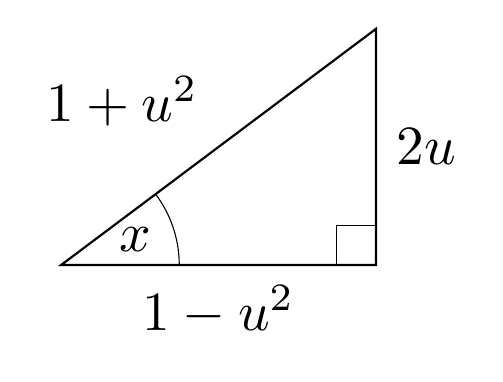
\begin{tikzpicture}[every node/.style = {scale = 2}]
\draw[thick] (0,0) -- node[pos = 0.5, below] {$1-u^2$} (4,0) -- node[pos = 0.5, right] {$2u$} (4,3) -- node[pos = 0.5, above left] {$1+u^2$} cycle;
\draw (1.5,0) arc [start angle = 0, end angle = 37, radius = 1.5] ;
\draw (4,0) rectangle (3.5, 0.5);
\node at (18.5: 1) {$x$};
\end{tikzpicture}
\end{column}
\end{columns}
\begin{slide}
นอกจากนั้น จาก $u = \tan \frac{x}{2}$ จะได้ $x = 2 \arctan u$ ดังนั้น
\[dx = 2 \left(\frac{1}{1+u^2} \right)\, du = \frac{2}{1+u^2} \, du \]
สุดท้ายแล้วพจน์ฟังก์ชันตรีโกณมิติและพจน์ $dx$ จะกลายเป็นตัวแปร $u$ ทั้งหมด
\end{slide}
\end{frame}

\begin{frame}
\begin{remark}{เทคนิคการใช้สูตรมุมครึ่ง}
กำหนดให้ $u = \tan \frac{x}{2}$ แล้วจะได้
\begin{eq*}
\sin x &=& \frac{2u}{1+u^2} \\
\cos x &=& \frac{1-u^2}{1+u^2} \\
dx &=& \frac{2}{1+u^2} \, du
\end{eq*}
\end{remark}
\end{frame}


\begin{frame}[t]
\begin{ex}
จงหาปริพันธ์ $\int \frac{1}{1 + \cos x + \sin x} \, dx$
\end{ex}
\begin{sol}
กำหนดตัวแปรใหม่ ให้ $u = \tan \frac{x}{2}$ และแปลงค่า $\sin x, \cos x, \, dx$ ให้เป็น $u$ ตามที่กำหนดไว้ จะได้
\begin{eqnarray*}
1 + \cos x + \sin x &=& 1 + \frac{1-u^2}{1+u^2} + \frac{2u}{1+u^2} \\
&=& \frac{(1+u^2) + (1-u^2) + (2u)}{1+u^2} \\
&=& \frac{2+2u}{1+u^2}
\end{eqnarray*}
\end{sol}
\end{frame}

\begin{frame}[t]
\begin{sol} (ต่อ)
เมื่อแทนค่ากลับไปในปริพันธ์จะได้
\begin{eq*}
\int \frac{1}{1 + \cos x + \sin x} \, dx &=& \int \frac{1}{\left( \frac{2+2u}{1+u^2} \right)} \left(\frac{2}{1+u^2} \, du\right) \\
&=& \int \left(\frac{1+u^2}{2+2u}\right) \left( \frac{2}{1+u^2}\right) \, du \\
&=& \int \frac{1}{1+u} \, du \\
&=& \ln |1+u| + C \\
&=& \ln \left|1 + \tan \frac{x}{2} \right| + C 
\end{eq*}
\end{sol}
\end{frame}




\begin{frame}[t]
\begin{ex}
จงหาปริพันธ์ $\int \frac{1}{2 + \sin x} \, dx$
\end{ex}
\begin{sol}
กำหนดตัวแปรใหม่ ให้ $u = \tan \frac{x}{2}$ และแปลงค่า $\sin x, dx$ ให้เป็น $u$ ตามที่กำหนดไว้ จะได้
\begin{eqnarray*}
2 + \sin x &=& 2 + \frac{2u}{1+u^2} = \frac{2(1+u^2) + 2u}{1+u^2} = 2 \left( \frac{1+u+u^2}{1+u^2} \right) \\
dx &=& \frac{2}{1+u^2} \, du
\end{eqnarray*}
ฉะนั้น
\[\int \frac{1}{2+\sin x} \, dx = \int \frac{1}{2\left(  \frac{1+u+u^2}{1+u^2} \right)} \left( \frac{2}{1+u^2} \, du \right) = \int \frac{1}{u^2+u+1} \, du\]
\end{sol}
\end{frame}

\begin{frame}[t]
\begin{sol} (ต่อ)
เราสามารถหาปริพันธ์ $\int \frac{1}{u^2+u+1} \, du$ ได้ด้วยการใช้สูตรปริพันธ์ของ $\frac{1}{a^2+z^2}$ โดยการจัดรูปกำลังสองดังนี้
\[ u^2+u+1 = \left( u^2 + u + \frac{1}{4}\right) + \left(1 - \frac{1}{4}\right) = \left(u+\frac{1}{2}\right)^2 + \left( \frac{\sqrt{3}}{2} \right)^2 \]
ดังนั้น
\begin{eq*}
\int \frac{1}{u^2+u+1} \, du &=& \int \frac{1}{\left(u+\frac{1}{2}\right)^2 + \left( \frac{\sqrt{3}}{2} \right)^2} \, du \\
&=& \frac{1}{\left( \frac{\sqrt{3}}{2} \right)} \arctan \left( \frac{\sqrt{3}}{2} \left( u + \frac{1}{2} \right) \right) + C\\
&=& \frac{2}{\sqrt{3}} \arctan \left( \frac{2u+1}{\sqrt{3}} \right) = \frac{2}{\sqrt{3}} \arctan \left( \frac{1+\tan \frac{x}{2}}{\sqrt{3}} \right)
\end{eq*}
\end{sol}
\end{frame}

%%%%%%%%%%%%%%
\section[แทนค่าด้วยฟังก์ชันอื่น ๆ]{การหาปริพันธ์โดยการแทนค่าด้วยฟังก์ชันอื่น ๆ}
\frame{\sectionpage}
%%%%%%%%%%%%%%


\begin{frame}[t]
ถ้าเจอฟังก์ชันรูปแบบอื่น ๆ เราจะต้องใช้ประสบการณ์ในการลองผิดลองถูก ไม่มีรูปแบบตายตัว เช่น ถ้าเจอพจน์ $(ax+b)^{\frac{1}{n}}$ แล้วจะให้ $u = (ax+b)^{\frac{1}{n}}$ ทั้งพจน์ หรือ $u = ax+b$ ก็เป็นไปได้ทั้งคู่
\begin{ex}
จงหาปริพันธ์ $\int \frac{1}{x\sqrt{x-1}} \, dx$
\end{ex} \pa
\begin{sol}
ทดลองใช้การแทนค่า $u = x-1$ จะได้
\[\int \frac{1}{x\sqrt{x-1}} \, dx = \int \frac{1}{(u+1)\sqrt{u}} \, du\]
ซึ่งไม่ได้เปลี่ยนรูปแบบเท่าใด $\ldots$ เป็นเรื่องปกติที่ต้องทดลองหลาย ๆ ค่า
\end{sol}
\end{frame}

\begin{frame}[t]
\begin{sol} (ต่อ)
จึงทดลองใหม่โดยใช้ $u = \sqrt{x-1}$ จะได้ 
\[ u^2 = x-1 \qquad \rightarrow \qquad x = u^2+1\]
\[ x = u^2 + 1 \qquad \rightarrow \qquad dx = 2u \, du\]
ฉะนั้น
\begin{eq*}
\int  \frac{1}{x\sqrt{x-1}} \, dx &=& \int \frac{1}{(u^2+1) u} (2u \, du) \\
&=& 2 \int \frac{1}{u^2+1} \, du \\
&=& 2 \arctan u + C \\
&=& 2 \arctan \sqrt{x-1} + C
\end{eq*}
\end{sol}
\end{frame}


\begin{frame}[t]
\begin{ex}
จงหาปริพันธ์ $\int \sin \sqrt{x} \, dx$
\end{ex} \pa
\begin{sol}
ทดลองใช้การแทนค่า $u = \sqrt{x}$ จะได้ 
\[du = \frac{1}{2x} \, dx \qquad dx = 2x \, du\]
นอกจากนั้น เรายังได้ $x = u^2$ ฉะนั้น
\[\int \sin \sqrt{x} \, dx = \int \sin u (2x \, du) =2 \int u^2 \sin u \, du\] 
ซึ่งสังเกตว่า เป็นรูปแบบปริพันธ์ที่เราเคยหามาแล้ว นั่นคือการแยกส่วน
\end{sol}
\end{frame}


\begin{frame}[t]
\begin{sol} (ต่อ)
เมื่อหาปริพันธ์แยกส่วนจะได้
\begin{eq*}
\int \red{u^2} \blue{\sin u  \, du} &=& \red{u^2} \blue{(-\cos u)} - \int \blue{(-\cos u)}\red{(2u \, du)} \\
&=&-u^2\cos u + 2 \int u\cos u \, du \\
&=&-u^2 \cos u + 2( \green{u} \red{\sin u} - \int \red{\sin u} \, \green{du} ) \\
&=& -u^2 \cos u + 2u\sin u + 2\cos u + C
\end{eq*}
สุดท้าย เมื่อแทนค่า $u = \sqrt{x}$ จะได้ 
\[ \int \sin \sqrt{x} \, dx = -x \cos \sqrt{x} + 2\sqrt{x} \sin \sqrt{x} + 2 \cos \sqrt{x} + C\]
\end{sol}
\end{frame}
